
\section{作用量-角坐标，阿诺德-约斯特定理}
\label{sec:action-angle-arnold-jost}

\hzsync{theorem}{2}%
\hzsync{lemma}{2}%
\hzsync{equation}{17}%

我们考虑一个 $\dim M=2n$ 的\trSymplecticManifold{} $(M,\omega)$。

\textbf{\trhDefinition。}\quad $M$ 上的一个\trHamiltonianVectorField{} $X_{H}$ 称为可积的%
（\trLiouville{}意义下），若存在 $n$ 个函数 $F_{j}:M\to\R$，$1\leq j\leq n$，%
在 $M$ 的每一点处满足：
\[
\begin{array}{lll}
\text{(i)}   &\ dF_{1},\dots,dF_{n}\ \text{线性无关} &\\
\text{(ii)}  &\ \{F_{i},F_{j}\}=0 &\ \text{对一切 }i,\ j\,.\\
\text{(iii)} &\ \{H,F_{j}\}=0 &\ \text{对一切 }j\,.
\end{array}
\]

引入映射
\begin{equation}\label{eq:action-map}
F:M\longrightarrow\R^{n}\,,\qquad F(x)=\bigl(F_{1}(x),\dots,F_{n}(x)\bigr)
\end{equation}
并由 (i) 得知诸\trLevelSet
\begin{equation}\label{eq:level-sets}
N_{c}=\bigl\{\,x\in M\ \bigm|\ F(x)=c\,\bigr\}\,,\qquad c\in\R^{n}
\end{equation}
是 $M$ 的 $n$ 维\trSubmanifold。诸\trHamiltonianVectorField{} $X_{F_{j}}$ 是%
\trLinearlyIndependent{}的，而且由于据 (ii) 有 $dF_{i}(X_{F_{j}})=0$，它们张成 $N_{c}$ 的%
\trTangentSpace：
\[
T_{x}N_{c}=\operatorname{span}\{\,X_{F_{j}}(x)\mid 1\leq j\leq n\,\}\,,\qquad x\in N_{c}.
\]
此外我们还注意到，由 $\omega(X_{F_{j}},X_{F_{i}})=0$ 可知，对每一对%
$v$, $w\in T_{x}N_{c}$ 都有 $\omega(v,w)=0$。故 $N_{c}$ 是 $M$ 的一个%
\trLagrange{}\trSubmanifold。由 (iii)，诸函数 $F_{j}$ 全都是 $X_{H}$ 的\trFirstIntegral，%
因而 $X_{H}$ 与诸\trLevelSet{} $N_{c}$ 相切，于是 $X_{H}$ 的\trFlow{}使 $N_{c}$ 保持%
\trInvariant。对 $N_{c}$ 再附加一个\trTopology{}假设，借助于下述定理，这个\trFlow{}%
便可对一切时刻显式确定；该定理在特殊情形 $M=\R^{2n}$ 下可追溯至%
V.~\trArnold{} [12]。然而，\trArnold{}当时需要一个附加假设，该假设后来由%
R.~\trJost{}在 [126] 中去除，他并在一般情形下证明了这一定理。

\begin{theorem}[\trArnold-\trJost]\label{thm:arnold-jost}
设 $(M,\omega)$ 是 $\dim M=2n$ 的\trSymplecticManifold。假设存在 $n$ 个在每一点处%
满足 (i) 与 (ii) 的函数 $F_{j}$。再假设其中一个\trLevelSet，比如说%
$N=F^{-1}(0)\subset M$，是\trCompact{}而且\trConnected{}的。那么

1) $N$ 是一个\trEmbedding{}的 $n$ 维\trTorus{} $T^{n}$。

2) 在 $M$ 中存在 $N$ 的一个开\trNeighborhood{} $U$，它可由\trAction{}与角变量%
$(x,y)$ 按下述方式描述。若 $x=(x_{1},\dots,x_{n})$ 是\trTorus{}%
$T^{n}=\R^{n}/\Z^{n}$ 上的变量，而 $y=(y_{1},\dots,y_{n})\in D_{1}$，其中 $D_{1}$%
与 $D_{2}$ 是 $\R^{n}$ 中包含 $y=0$ 的两个\trDomain，则存在一个\trDiffeomorphism
\[
\psi:T^{n}\times D_{1}\longrightarrow U=\bigcup_{c\in D_{2}}\bigl(F^{-1}(c)\cap U\bigr)
\]
与一个\trDiffeomorphism{} $\mu:D_{2}\to D_{1}$，$\mu(0)=0$，使得
\begin{equation}\label{eq:psi-star-omega}
\psi^{*}\omega=\sum_{j=1}^{n}dy_{j}\wedge dx_{j}=\omega_{0}
\end{equation}
\begin{equation}\label{eq:mu-F-psi}
\mu\circ F\circ\psi(x,y)=y\,.
\end{equation}
特别地，$\psi$ 把\trTorus{} $T^{n}\times\{0\}$ \trDiffeomorphism{}地映到%
$F^{-1}(0)=N$ 上，而把\trTorus{} $T^{n}\times\{y\}$ 映到 $N_{c}\cap U$ 上，%
其中 $y=\mu(c)$。
\end{theorem}

\textbf{\trhCorollary：}\quad 由 $H$ 给出的、具有诸\trFirstIntegral{} $F_{j}$ 的任一可积%
\trHamiltonianSystem，经\trSymplecticDiffeomorphism{} $\psi$ 变换为%
$(T^{n}\times D_{1},\omega_{0})$ 上的下述系统：
\begin{equation}\label{eq:h-of-psi}
H\circ\psi(x,y)=h(y)\,,
\end{equation}
其中\trHamiltonianFunction{} $h$ 只依赖于诸\trFirstIntegral{}而不依赖于角变量 $x$。

\begin{proof}[\trhCorollary{}的\trhProof]
据 \eqref{eq:a13-invariance}，诸函数 $F_{j}\circ\psi$，从而据 \eqref{eq:mu-F-psi}%
亦即诸坐标函数 $y_{j}$，%
都是 $H\circ\psi$ 的\trFirstIntegral，于是
\[
0=\{H\circ\psi,y_{j}\}=\{h,y_{j}\}=\frac{\partial}{\partial x_{j}}h
\]
故 $h(x,y)=H\circ\psi(x,y)$ 确实不依赖于诸 $x$ 变量。
\end{proof}

因而在 $\psi^{-1}(U)$ 上，变换后的\trHamiltonianSystem{}显得极为简单：
\[
X_{h}\ :\qquad \dot{x}=\frac{\partial h}{\partial y}(y)\,,\qquad \dot{y}=0\,.
\]
它容易被「积分」，其解为
\[
x(t)=x(0)+t\,\frac{\partial h}{\partial y}\bigl(y(0)\bigr)\,,\qquad y(t)=y(0)
\]
故有「可积系统」之名。几何上，$T^{n}\times D_{1}$\footnote{原书印作%
「$T^{n}\times D_{2}$」，疑为「$D_{1}$」之误——上文推论中经 $\psi$ 变换后的%
系统正定义在 $\bigl(T^{n}\times D_{1},\omega_{0}\bigr)$ 上，此处径改。%
——译者注}中的每一个\trTorus{}%
$T^{n}\times\{y\}$ 在 $X_{h}$ 的\trFlow{} $\varphi^{t}$ 之下都是\trInvariant{}的，%
而限制到这样一个\trTorus{}上是线性的：
\[
\varphi^{t}\big|_{T^{n}\times\{y\}}\ :\quad(x,y)\mapsto(x+t\omega,y)
\]
其中 $\omega=\frac{\partial h}{\partial y}(y)\in\R^{n}$ 是这一特定\trTorus{}的诸频率。%
我们看到，在开集 $U\subset M$ 中，$\dot{x}=X_{H}(x)$ 的一切解都是%
\trQuasiPeriodic{}的。

\begin{proof}[\cref*{thm:arnold-jost}的证明]
证明分几步进行。首先我们证明 $N$ 是一个\trTorus。其次，借助\trLiouville{}定理，%
我们在 $N$ 上一点 $p$ 附近引入便利的坐标 $(x,y)$。第三步，借助诸%
\trHamiltonianVectorField{} $X_{F_{j}}$ 的\trFlow{}把这些坐标延拓到 $N$ 的一个开%
\trNeighborhood{}上。最后，为结束证明，\trPeriodic{}的规范化尚需一个附加的%
\trSymplectic{}变量替换。

a) 为证明定理的第一条结论，我们以 $\varphi^{s}_{j}$ 记 $X_{F_{j}}$ 的\trFlow。%
由于 $[X_{F_{j}},X_{F_{i}}]$ 是以 $\{F_{i},F_{j}\}=0$ 为\trHamiltonianFunction{}的%
一个\trHamiltonianVectorField，诸\trVectorField{} $X_{F_{j}}$ 从而它们的\trFlow{}确实可交换，%
我们把它简写为
\begin{equation}\label{eq:flow-phi-s}
\varphi^{s}=\varphi^{s_{1}}_{1}\circ\varphi^{s_{2}}_{2}\circ\dots\varphi^{s_{n}}_{n}\,,%
\qquad s=(s_{1},\dots,s_{n})\in\R^{n}\,,
\end{equation}
只要它有定义。由于诸 $F_{j}$ 是 $X_{F_{i}}$ 的\trFirstIntegral，
\[
F\bigl(\varphi^{s}(x)\bigr)=F(x)\,,\qquad x\in M
\]
从而 $\varphi^{s}$ 使所有\trLevelSet{} $N_{c}\subset M$ 保持\trInvariant。%
现在取定一点 $p\in N$。由于 $N$ 是\trCompact{}的，\trFlow{} $\varphi^{s}(p)$%
对一切 $s\in\R^{n}$ 存在，于是我们可以定义 $\R^{n}$ 在 $N$ 上的\trGroupAction
\begin{equation}\label{eq:action-A}
A:\R^{n}\longrightarrow N,\qquad s\mapsto\varphi^{s}(p)\,.
\end{equation}
显然 $\varphi^{s}\circ\varphi^{t}=\varphi^{s+t}$。映射 $A$ 是一个\trImmersion，%
这是因为在 $t$ 处的切映射把 $e_{j}\in\R^{n}$ 映为%
$X_{F_{j}}\bigl(\varphi^{t}(p)\bigr)\in T_{\varphi^{t}(p)}N$，从而这些向量张成%
\trTangentSpace。%
因此 $A$ 是一个局部\trDiffeomorphism，其像既开又闭，从而等于 $N$，%
因为已设 $N$ 是\trConnected{}的。然而映射 $A$ 不是\trInjective。\trIsotropyGroup%
$\Gamma=\{s\in\R^{n}\mid\varphi^{s}(p)=p\}$ 是 $\R^{n}$ 的一个离散子群，%
即一个\textbf{\trLattice}（lattice）。于是 $\Gamma$ 由在 $\R$ 上\trLinearlyIndependent{}的%
向量 $\gamma_{1},\dots,\gamma_{d}\in\R^{n}$ 生成，并且
\begin{equation}\label{eq:lattice-gamma}
\Gamma=\Bigl\{\,\gamma=\sum_{j=1}^{d}n_{j}\gamma_{j}\ \Bigm|\ n_{j}\in\Z\,\Bigr\}\,.
\end{equation}
由 $\varphi^{s+\gamma}(p)=\varphi^{s}(p)$ 对一切 $s\in\R^{n}$ 成立，映射 $A$%
诱导出 $\R^{n}/\Gamma$ 与 $N$ 之间的一个\trDiffeomorphism。由于 $N$ 从而%
$\R^{n}/\Gamma$ 是\trCompact{}的，必有 $d=n$，故如所断言，$N$ 是一个 $n$ 维\trTorus。

b) 接着我们在点 $p\in N$ 附近引入便利的局部坐标。据\trDarboux{}定理与%
\trLiouville{}定理及其推论，我们有
\begin{lemma}[\trLiouville]\label{lem:liouville-coordinates}
若 $(M,\omega)$ 是 $\dim M=2n$ 的\trSymplecticManifold，而 $F_{j}$ 是 $n$ 个%
满足 $\{F_{j},F_{i}\}=0$ 且 $dF_{j}$ 处处\trLinearlyIndependent{}的函数，%
则每一点 $q\in M$ 都有开\trNeighborhood{} $W$ 与一个\trDiffeomorphism{}%
$\psi:V\to W$，其中 $V$ 是 $\R^{2n}$ 中原点的一个开\trNeighborhood，使得
\[
\begin{array}{lll}
\text{(i)}   &\ \psi(0)=q &\\
\text{(ii)}  &\ \psi^{*}\omega=\displaystyle\sum_{j=1}^{n}dy_{j}\wedge dx_{j}\,. &\\
\text{(iii)} &\ F\circ\psi(x,y)=y\,, &
\end{array}
\]
其中 $(x,y)$ 是 $(\R^{2n},\omega_{0})$ 的\trSymplecticCoordinates。
\end{lemma}

\textbf{\trhCorollary。}\quad 在上述「\trLiouville」坐标中，\eqref{eq:flow-phi-s}%
中定义的\trFlow{} $\varphi^{s}$ 显得非常简单，即
\begin{equation}\label{eq:liouville-flow}
\varphi^{s}\circ\psi(x,y)=\psi(x+s,y)\,,\qquad s\in\R^{n}
\end{equation}
只要 $(x,y)$ 与 $(x+s,y)\in V$。

的确，对每个 $1\leq j\leq n$，$\psi^{-1}\circ\varphi^{s}_{j}\circ\psi$ 是%
\trHamiltonianVectorField{} $X_{F_{j}\circ\psi}$ 在 $V$ 上的\trFlow。由于%
$F_{j}\circ\psi(x,y)=y_{j}$，它确实是线性的，并由%
$(x,y)\mapsto(x+s_{j}e_{j},y)$ 给出。

c) 回到我们的点 $p\in N$。据\cref{lem:liouville-coordinates}选取\trLiouville{}坐标%
$\psi:V\to U\subset M$，其中 $V$ 是 $\R^{2n}$ 中 $0$ 的一个开\trNeighborhood{}%
而 $\psi(0)=p$。为把这些坐标延拓到 $(x,y)\in\R^{2n}$，我们将定义一个映射
\begin{equation}\label{eq:vartheta-def}
\begin{aligned}
\vartheta:\qquad &\R^{n}\times D_{2}\longrightarrow M\\
&(x,y)\longmapsto\vartheta(x,y)=\varphi^{x}\circ\psi(0,y)
\end{aligned}
\end{equation}
其中 $\varphi^{x}$ 是 \eqref{eq:flow-phi-s} 中定义的由诸\trVectorField{} $X_{F_{j}}$ 生成的%
可交换\trFlow，而 $D_{2}\subset\R^{n}$ 是 $y=0$ 的一个开（而且小）的\trNeighborhood。%
对小的 $x$，据上述推论我们有 $\vartheta(x,y)=\psi(x,y)$，对 $(x,y)\in V$ 成立。%
几何上，定义 \eqref{eq:vartheta-def} 是说，我们把\trFlow{} $\varphi^{x}$ 作用到%
局部\trSection{} $S=\{\psi(0,y)\in M:y\in D_{2}\}$ 上，而据上述推论，%
这个\trSection{}与诸\trVectorField{} $X_{F_{j}}$ \trTransversal。

\noindent\begin{minipage}{\linewidth}
\centering
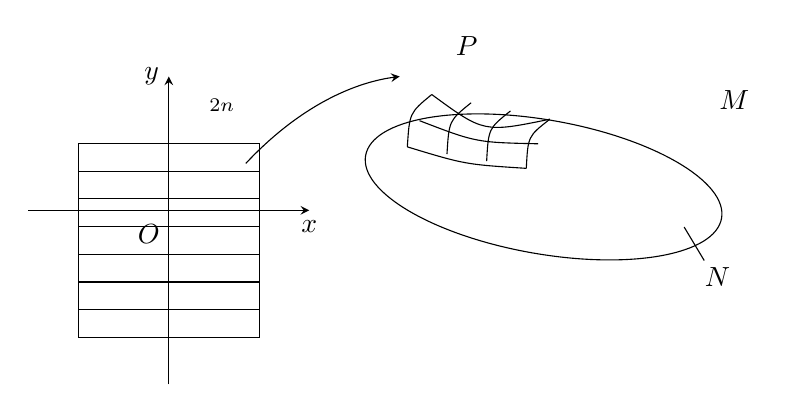
\begin{tikzpicture}[>=stealth,scale=0.85]
  \draw[->] (-2.1,0) -- (2.1,0) node[below] {$x$};%
  \draw[->] (0,-2.6) -- (0,2.0) node[left] {$y$};%
  \node at (-0.3,-0.35) {$O$};
  \draw (-1.35,-1.9) rectangle (1.35,1.0);%
  \foreach \i in {1,...,6}
    \draw (-1.35,-1.9+0.4143*\i) -- (1.35,-1.9+0.4143*\i);%
  \node at (0.8,1.5) {$\R^{2n}$};
  \draw[->] (1.15,0.7) .. controls (1.9,1.5) and (2.7,1.9) .. (3.45,2.0);%
  \begin{scope}[rotate around={-10:(5.6,0.35)}]
    \draw (5.6,0.35) ellipse [x radius=2.7, y radius=1.0];%
  \end{scope}
  \begin{scope}[shift={(4.55,1.15)},rotate=-15]
    \draw (-0.9,-0.45) .. controls (-1.0,0.05) .. (-0.75,0.4);%
    \draw (0.9,-0.3) .. controls (0.8,0.17) .. (1.05,0.5);%
    \draw (-0.9,-0.45) .. controls (0.0,-0.48) .. (0.9,-0.3);%
    \draw (-0.75,0.4) .. controls (0.15,0.05) .. (1.05,0.5);%
    \draw (-0.3,-0.4) .. controls (-0.4,0.09) .. (-0.15,0.433);%
    \draw (0.3,-0.35) .. controls (0.2,0.13) .. (0.45,0.467);%
    \draw (-0.825,-0.025) .. controls (0.075,-0.12) .. (0.975,0.1);%
  \end{scope}
  \node at (4.45,2.45) {$P$};
  \node at (8.45,1.65) {$M$};
  \draw (7.7,-0.25) -- (8.0,-0.75);%
  \node at (8.2,-1.0) {$N$};
\end{tikzpicture}

图 A2.1
\end{minipage}

此外，由于 $F\circ\varphi^{x}=F$，我们从\cref{lem:liouville-coordinates}（iii）%
得出 $F\bigl(\vartheta(x,y)\bigr)=F\bigl(\varphi^{x}\circ\psi(0,y)\bigr)=%
F\bigl(\psi(0,y)\bigr)=y$，从而
\begin{equation}\label{eq:vartheta-level}
\vartheta:\R^{n}\times\{y\}\longrightarrow N_{y}=F^{-1}(y)
\end{equation}
对 $y\in D_{2}$ 在该映射有定义之处成立。若 $y=0$，则由 $\psi(0,0)=p$ 得%
$\vartheta(x,0)=\varphi^{x}(p)$，于是据 a) 中的考虑，该映射对一切 $x\in\R^{n}$%
有定义，并把 $\R^{n}\times\{0\}$ 映满 $N=F^{-1}(0)$。由此可见，只要 $D_{2}$%
足够小，$\vartheta$ 便定义在 $K\times D_{2}$ 上，其中 $K\subset\R^{n}$ 是%
一个内部含有\trLattice{} $\Gamma$ 之基本平行多面体的\trCompact{}集\footnote{原书%
此处及\cref{lem:vartheta-global}的证明中两度印作「内部含有格 $\Gamma$（后者作%
$\Gamma(0)$）的紧集」：满秩格无界，不可能含于任何紧集之内；核其论证，所需者%
仅为此紧集的内部含有格的一个基本平行多面体（一切 $x\in\R^{n}$ 均可写成格点与%
此多面体中一点之和，且对充分小的 $y$ 于 $\Gamma(y)$ 一致成立），两处均径改。%
——译者注}。下面我们将证明 $\vartheta$ 实际上%
定义在整个 $\R^{n}\times D_{2}$ 上。回顾一下：若 $y=0$，则对 $x\in\R^{n}$ 与%
$\gamma\in\Gamma$ 有 $\vartheta(x+\gamma,0)=\vartheta(x,0)$。我们将先对 $0$ 的%
一个小\trNeighborhood{}内的 $y$ 构造一个靠近 $\Gamma(0)=\Gamma$ 的 $n$ 维\trLattice%
$\Gamma(y)\subset\R^{n}$，使得对每个 $\gamma(y)\in\Gamma(y)$ 都有%
$\vartheta\bigl(x+\gamma(y),y\bigr)=\vartheta(x,y)$。

设 $\gamma=\gamma_{j}\in\Gamma$ 是 \eqref{eq:lattice-gamma} 中所定义\trLattice{}的%
一个任意基向量。则 $\varphi^{\gamma}(p)=p$ 而 $p=\psi(0)$。于是，在%
\trLiouville{}坐标 $V\subset\R^{2n}$ 中
\begin{equation}\label{eq:psi-conjugate}
\psi^{-1}\circ\varphi^{\gamma}\circ\psi\ :\ (x,y)\mapsto(\xi,\eta)
\end{equation}
在 $V$ 中\trFixedPoint{} $0$ 附近局部地定义了一个\trSymplecticDiffeomorphism。

\begin{lemma}\label{lem:gamma-translation}
\eqref{eq:psi-conjugate} 中的\trSymplectic{}映射在 $V$ 中形如
\begin{equation}\label{eq:gamma-map-form}
\begin{aligned}
\xi\ &=\ x-v(y)\,,\qquad v(y)=\frac{\partial}{\partial y}Q(y)\,,\\
\eta\ &=\ y
\end{aligned}
\end{equation}
其中 $Q$ 是满足 $Q(0)=0$ 的一个\trSmooth{}标量函数。此外，$v(0)=0$。
\end{lemma}

\begin{proof}
由于按定义 $\varphi^{\gamma}\circ\psi(x,y)=\psi(\xi,\eta)$，我们由%
$F\circ\varphi^{x}=F$ 并据\cref{lem:liouville-coordinates}（iii）\footnote{原书%
此处印作「（ii）」，且链之首二项印作 $F\circ\psi(x,\eta)$、$F\circ\varphi^{\gamma}\circ%
\psi(x,\eta)$：$F\circ\psi(x,y)=y$ 系 (iii) 之结论（(ii) 为辛标准形式条件），%
链中之 $\eta$ 系 $y$ 之误（$\varphi^{\gamma}\circ\psi$ 之自变量为 $(x,y)$，$\eta$%
正待此链确定），均径改。——译者注}得出
\[
y=F\circ\psi(x,y)=F\circ\varphi^{\gamma}\circ\psi(x,y)=%
F\circ\psi(\xi,\eta)=\eta\,.
\]
每一个延拓关系 $\eta=y$ 的\trSymplectic{}映射都必然具有上述形式，%
这一点我们已在上一节见到。$v(0)=0$ 则由 $\psi^{-1}\circ\varphi^{\gamma}\circ%
\psi(0)=0$ 得出。
\end{proof}

按定义 \eqref{eq:psi-conjugate} 有 $\varphi^{\gamma}\circ\psi(x,y)=\psi(\xi,\eta)$，%
从\cref{lem:gamma-translation}与\cref{lem:liouville-coordinates}得出
\begin{equation}\label{eq:psi-gamma-v}
\psi(x,y)=\varphi^{\gamma+v(y)}\circ\psi(x,y)
\end{equation}
对 $(x,y)\in V'\subset V$ 成立。我们可以对每个基向量 $\gamma_{j}\in\Gamma$%
如法炮制，找到 $v_{j}(y)=\frac{\partial}{\partial y}Q_{j}(y)$，使得把%
$\gamma+v(y)$ 换成 $\gamma_{j}+v_{j}(y)$ 后 \eqref{eq:psi-gamma-v} 仍然成立。%
因此我们引入\trLattice{} $\Gamma(y)\subset\R^{n}$ 如下：
\begin{equation}\label{eq:lattice-gamma-y}
\Gamma(y)=\Bigl\{\,\gamma(y)=\sum_{j=1}^{n}n_{j}\gamma_{j}(y)\ \Bigm|\ n_{j}\in\Z\,\Bigr\}
\end{equation}
其中，据\cref{lem:gamma-translation}，
\[
\gamma_{j}(y)=\gamma_{j}+v_{j}(y)=\frac{\partial}{\partial y}W_{j}(y)\,,%
\qquad 1\leq j\leq n\,.
\]
此处 $\gamma_{j}\in\Gamma$，而诸 $W_{j}$ 是满足 $W_{j}(0)=0$ 的标量函数。%
此外，由于 $v_{j}(0)=0$，我们有 $\gamma_{j}(0)=\gamma_{j}$，从而
\begin{equation}\label{eq:gamma-zero}
\Gamma(0)=\Gamma\,.
\end{equation}
于是，对小的 $y$，\trLattice{}向量 $\gamma_{j}(y)$ 是\trLinearlyIndependent{}的，并且据%
\eqref{eq:psi-gamma-v} 满足
\begin{equation}\label{eq:psi-gammaj}
\psi(x,y)=\varphi^{\gamma_{j}(y)}\circ\psi(x,y)\,,\qquad 1\leq j\leq n\,,
\end{equation}
只要 $(x,y)\in V'\subset V$。

\begin{lemma}\label{lem:vartheta-global}
\eqref{eq:vartheta-def} 中定义的映射 $\vartheta:(\R^{n}\times D_{2},\omega_{0})%
\to(M,\omega)$ 对一切 $(x,y)\in\R^{n}\times D_{2}$ 存在，并且满足
\[
\begin{array}{ll}
\text{(i)}  &\ \vartheta^{*}\omega=\omega_{0}\,.\\
\text{(ii)} &\ \vartheta\bigl(x+\gamma(y),y\bigr)=\vartheta(x,y)\,,%
\quad \text{若 }\gamma(y)\in\Gamma(y)\,.
\end{array}
\]
\end{lemma}

\begin{proof}
只要 $D_{2}$ 足够小，映射 $\vartheta$ 便在 $(x,y)\in K\times D_{2}$ 上存在，%
其中 $K\subset\R^{n}$ 是内部含有 $\Gamma(0)$ 之基本平行多面体的\trCompact{}集。%
由于对小的 $x$，%
据 \eqref{eq:psi-gammaj}，
\begin{align*}
\vartheta\bigl(x+\gamma_{j}(y),y\bigr)\ &=\ \varphi^{x+\gamma_{j}(y)}\circ\psi(0,y)\\
&=\ \varphi^{x}\circ\varphi^{\gamma_{j}(y)}\circ\psi(0,y)\\
&=\ \varphi^{x}\circ\psi(0,y)\ =\ \vartheta(x,y)
\end{align*}
对每个 $\gamma_{j}(y)\in\Gamma(y)$ 成立，\trFlow{} $x\mapsto\varphi^{x}\circ\psi(0,y)$%
便确实对一切 $x\in\R^{n}$ 存在，这里依据的是常\trDifferentialEquation{}之解的标准延拓定理。%
剩下只需证明 (i)。若 $(x,y)\in\R^{n}\times D_{2}$，我们选取靠近 $x$ 的 $x_{0}$%
使 $(x-x_{0},y)\in V$，并把映射 $\vartheta$ 表示为
\begin{align*}
\vartheta(x,y)\ &=\ \varphi^{x_{0}+(x-x_{0})}\circ\psi(0,y)\\
&=\ \varphi^{x_{0}}\circ\psi(x-x_{0},y)\ =\ \varphi^{x_{0}}\circ\psi\circ\sigma_{x_{0}}(x,y)
\end{align*}
其中 $\sigma_{x_{0}}(x,y)=(x-x_{0},y)$，而且我们用到了%
\cref{lem:liouville-coordinates}之推论。于是，$\vartheta$ 局部地是诸%
\trSymplectic{}映射的复合，确实是\trSymplectic{}的，引理得证。
\end{proof}

回顾 $\vartheta\bigl(\R^{n}\times\{y\}\bigr)\subset F^{-1}(y)$。我们断言：%
对每个 $y\in D_{2}$，映射 $\vartheta$ 诱导出一个到其在 $F^{-1}(y)$ 中的像上的%
\trDiffeomorphism
\begin{equation}\label{eq:vartheta-quotient}
\vartheta_{0}:\R^{n}/\Gamma(y)\longrightarrow F^{-1}(y)
\end{equation}
而这个像便是一个\trTorus{} $T^{n}$。我们只需证明：只要 $y$ 充分小，%
$\vartheta_{0}$ 就是\trInjective。用反证法，设有序列 $(x_{j},y_{j})$ 与%
$(x'_{j},y_{j})$ 满足
\begin{equation}\label{eq:contradiction-sequences}
\begin{aligned}
&\vartheta(x_{j},y_{j})=\vartheta(x'_{j},y_{j})\,,\qquad y_{j}\to 0\\
&x_{j}-x'_{j}\notin\Gamma(y_{j})\,.
\end{aligned}
\end{equation}
取一个子列，可设 $x_{j}\to x^{*}$ 且 $x'_{j}\to x'^{*}$。于是%
$\vartheta(x^{*},0)=\vartheta(x'^{*},0)$，从而 $x^{*}-x'^{*}\in\Gamma(0)=\Gamma$。%
因此 $x_{j}-x'_{j}$ 靠近 $\Gamma(y_{j})$ 中的一点。由于 $\Gamma(y)$ 离散，%
且点与点之间的距离对 $y$ 一致地大于某个正常数，我们得出%
$x_{j}-x'_{j}\in\Gamma(y_{j})$。这与 \eqref{eq:contradiction-sequences} 矛盾，%
从而证明了断言 \eqref{eq:vartheta-quotient}。

d) 最后，我们借助另一个\trSymplecticDiffeomorphism{}来规范化诸\trLattice{} $\Gamma(y)$：
\begin{align*}
\sigma:\R^{n}\times D_{1}\ &\longrightarrow\ \R^{n}\times D_{2}\\
(\xi,\eta)\ &\longmapsto\ (x,y)\,.
\end{align*}
回顾 \eqref{eq:lattice-gamma-y} 中\trLattice{} $\Gamma(y)\subset\R^{n}$ 的定义，%
\trSymplectic{}映射 $\sigma$ 由\trGeneratingFunction{}隐式地定义：
\begin{equation}\label{eq:sigma-generating}
V(\xi,y)=\sum_{j=1}^{n}\xi_{j}W_{j}(y)\,;
\end{equation}
于是
\begin{equation}\label{eq:sigma-derivatives}
\begin{aligned}
\eta_{j}\ &=\ \frac{\partial}{\partial\xi_{j}}V(\xi,y)\ =\ W_{j}(y)\\
x_{j}\ &=\ \frac{\partial}{\partial y_{j}}V(\xi,y)\ =\ \sum_{s=1}^{n}\xi_{s}\,%
\frac{\partial}{\partial y_{j}}W_{s}(y)\,.
\end{aligned}
\end{equation}
\eqref{eq:sigma-derivatives} 中的第一个关系 $\eta=W(y)$ 在\trFixedPoint{} $y=0$%
附近定义了一个局部\trDiffeomorphism。在\cref*{thm:arnold-jost}的陈述中它记作%
$\mu:D_{2}\to D_{1}$。这由以下事实得出：
\[
\frac{\partial}{\partial y}W(y)=\bigl(\gamma_{1}(y),\dots,\gamma_{n}(y)\bigr)
\]
的\trRank{}为 $n$。的确，列向量 $\gamma_{j}(y)$ 正是 $\Gamma(y)$ 的 $n$ 个%
\trLinearlyIndependent{}的生成元。故 $\det(V_{\xi y})=\det W_{y}\neq0$\footnote{%
原书印作「$\det(V_{\xi})\neq0$」：$V_{\xi}=W(y)$ 是向量，无从取行列式，疑漏排%
一双下标，应为 $\det(V_{\xi y})=\det W_{y}\neq0$，此处径改。——译者注}。此外，当 $\eta=\mu(y)$%
时 $\sigma(e_{j},\eta)=\bigl(\gamma_{j}(y),y\bigr)$，从而
\[
\sigma:\Z^{n}\times\{\eta\}\longrightarrow\Gamma(y)\times\{y\}\,,%
\qquad \eta=\mu(y)\,.
\]
复合
\[
\Phi:=\vartheta\circ\sigma\ :\ (\R^{n}\times D_{1},\omega_{0})%
\longrightarrow(M,\omega)
\]
是一个\trSymplectic{}映射，满足 $\Phi(\xi+e_{j},\eta)=\Phi(\xi,\eta)$。%
它诱导出一个\trSymplecticDiffeomorphism
\[
\Phi:\R^{n}/\Z^{n}\times D_{1}\longrightarrow U\subset M
\]
这正是定义\trAction{}与角变量（记作 $(\xi,\eta)\in T^{n}\times D_{1}$）所需的映射。%
的确，利用这些定义我们算得 $\mu\circ F\circ\Phi(\xi,\eta)=%
\mu\circ F\circ\vartheta\circ\sigma(\xi,\eta)=\mu\circ F\circ\vartheta(x,y)=%
\mu(y)=\eta$，正如\cref*{thm:arnold-jost}所断言的那样，该定理的证明至此完成。
\end{proof}

\trSymplecticManifold{} $(M,\omega)$ 不必是\trExact{}的（\trExact{}意指%
$\omega=d\alpha$，$\alpha$ 是 $M$ 上的一个\trOneForm\footnote{原书于此段以%
$\vartheta$、$\sigma$ 名此两个\trOneForm，与 \eqref{eq:vartheta-def} 所定义之映射%
$\vartheta$ 及前 d) 中之映射 $\sigma$ 重名；为免类型混淆，译文分别改作 $\alpha$%
与 $\beta$。——译者注}）。但从%
\cref*{thm:arnold-jost}可知，把 $\omega$ 限制到\trActionAngle{}坐标在 $M$ 中的像%
$U=\psi(T^{n}\times D)$ 上，便得到一个\trExact{}形式。的确，$\omega\big|_{U}=d\beta$，%
其中\trOneForm{} $\beta=(\psi^{-1})^{*}\lambda$，而 $\lambda=\sum_{j=1}^{n}y_{j}\,dx_{j}$%
在 $T^{n}\times D$ 上满足 $d\lambda=\omega_{0}$。这使我们能够把\trAction{}变量%
$y=\mu\circ F$ 取作 $\beta$ 沿 $N_{c}\cap U$ 上的\trClosed\trCurve{}的%
「作用量积分」，这些闭曲线的\trHomology{}类构成 $H_{1}(N_{c}\cap U,\Z)$ 中的%
一组基，且 $\mu(c)=y$\footnote{原书印作「$\mu(x)=y$」，其 $x$ 系能级参数 $c$ 之误%
（$\mu:D_{2}\to D_{1}$ 以 $c$ 为自变量，于 $N_{c}$ 上 $y=\mu(c)$），此处径改。%
——译者注}。故有「\trAction{}变量」之名。


我们构造出的\trActionAngle{}变量 $(x,y)$ 当然不是唯一的。给定一个%
\textbf{\trUnimodular}（unimodular）矩阵 $M\in GL(n,\Z)$、一个函数 $w(y)$ 与一组%
常数 $c\in\R^{n}$，借助 $T^{n}\times D$ 的下述\trSymplecticDiffeomorphism，%
我们便找到另一组\trActionAngle{}变量 $(x',y')$：
\begin{align*}
x' &= M\Bigl(x+\frac{\partial w}{\partial y}(y)\Bigr)\\
y' &= \bigl(M^{T}\bigr)^{-1}y+c\,.
\end{align*}
这相当于用矩阵 $M$ 更换 $T^{n}$ 的\trFundamentalGroup{}的一组基，并对诸%
角变量施以一个\trPhaseShift{} $\frac{\partial w}{\partial y}(y)$\footnote{原书印作%
「对诸作用量变量施以相移」：式中 $\frac{\partial w}{\partial y}(y)$ 系加于%
角变量 $x$ 之上（$y$ 才是作用量变量），疑为「角变量」之误，此处径改。%
——译者注}。$T^{n}$ 上的%
直线在此映射下被映为直线。

我们已在一个\trTorus{}附近构造了\trActionAngle{}坐标，人们自然会问：这些%
局部的\trActionAngle{}坐标卡是如何拼合在一起的。我们不讨论这个整体性问题，%
而是转而请读者参见 N.~\trNekhoroshev{} [168]（1972）、A.~S.~\trMishchenko{}与%
A.~T.~\trFomenko{} [158]（1978），特别是 J.~J.~\trDuistermaat{} [64]（1980）。%
可积系统构成\trHamiltonianSystem{}中一个非常受限、甚至例外的类。若干例子%
在注记 [167] 中有所描述，本附录即取材于它，仅作了少量修改。关于可积系统%
领域中令人关注的新进展，我们请读者参见 J.~\trMoser{} [166]。
